\scanpage{183}
% archive foliation: 182
$\pi_0$
\figure{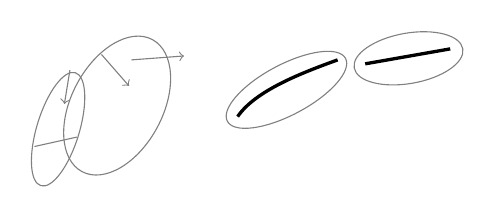
\begin{tikzpicture}[x=1cm,y=1cm]
\draw[gray,rotate around={-17:(.5,.6)}] (.5,.6) ellipse (.27 and .75);
\draw[gray,rotate around={-28:(1.25,.9)}] (1.25,.9) ellipse (.58 and .95);
\draw[gray,->] (.65,1.35)--(.58,.92);
\draw[gray,->] (1.05,1.55)--(1.40,1.15);
\draw[gray,->] (1.43,1.48)--(2.1,1.53);
\draw[gray] (.2,.38)--(.74,.5);
\draw[gray,rotate around={28:(3.4,1.1)}] (3.4,1.1) ellipse (.85 and .32);
\draw[very thick] (2.78,.76) .. controls (3.0,1.08) and (3.55,1.30) .. (4.05,1.48);
\draw[gray,rotate around={10:(4.95,1.5)}] (4.95,1.5) ellipse (.70 and .32);
\draw[very thick] (4.4,1.43)--(5.48,1.62);
\end{tikzpicture}}

\diagram{\begin{tikzcd}
F^0\arrow[r,shift left=.5ex]\arrow[r,shift right=.5ex]&
F^1\arrow[r,shift left=1ex]\arrow[r]\arrow[r,shift right=1ex]&F^2
\end{tikzcd}}
foncteurs $(\mathrm{Ens})\to(\mathrm{Ens})$

Objet simplicial de $\underline{\operatorname{Hom}}(\mathrm{Ens},\mathrm{Ens})$

Permet en principe de définir des $\pi_0,\pi_1$

$\pi_0(F)$, $F\in\underline{\operatorname{Hom}}(\mathrm{Ens},\mathrm{Ens})$, $F$
\[
F(I)\underset{?}{\simeq}C(K,I)
\]
$K$ espace top \uline{tot. discontinu}
[deux pts sont séparés par un ens : à la fois ouvert et fermé]

\uline{Cond néc} a) $F$ \unsure{permute|commute} aux
\deleted{produits} $\varprojlim$ finies

i.e. $F$ \uline{exact à gauche}
[donc $F$ transforme mon. en mon.]

b) \[
F(\bigcap I_\alpha)=\bigcap_\alpha F(I_\alpha)
\]
pour $(I_\alpha)$ famille filtrante de sous-ens. de $I$

Ces conditions équivalent à : \uline{$F$ strictement proreprésentable}
par un système projectif strict $(\pi_{0i})_i$ \deleted{\unsure{de}} d'ensembles.

Il faut de plus

c) \[
\deleted{\unsure{\pi_0F}}\quad
\varprojlim\pi_{0i}\longrightarrow\pi_{0i}
\quad\text{est \uline{surjectif} pour }\forall\,i.
\]

Ces conditions sont \uline{néc} et suffisantes, et on pourra prendre
$K=\varprojlim\pi_{0i}$, avec la topologie limite inverse des top. discrètes.

\uline{NB} Si $F$ est donné dans la forme $C(L,I)$, $L$ esp. top, homo
\[
\pi_0(L)\longrightarrow K.
\]
Si $L$ est \inserted{(quasi)} compact, cet homo est un
\unsure{isomorphisme|homéomorphisme}; \uline{en général}, ce n'est ni injectif, ni surjectif,

\margin{?\\Bourb. Topologie II\\p. 232, prop 6}
